%----------------------------------------------------------------------------
\chapter{Evaluation}
%----------------------------------------------------------------------------
\section{Displaying the imperative program}
During development, and when running the finished tool, it became very important to see the output of the parser part in an easy to read form. The C\# debugger did not fit for that job, since despite that I could see the object hierarchy, and inspect values and statements one-by-one, I could not see the converted program as a whole. 

Therefore, I overrode the ToString functions for all the model objects to return an easy to read string reflecting its contents. After that, all I had to do was to call ToString on a \textit{Sequence} object, and it returned a pseudo-code of the converted program.

In the following examples, the shown converted imperative examples are the output of this routine.
\section{Small demos}
\paragraph{Demo "A"}
For the first demo I used the same program, which I used to demonstrate symbolic execution in the Background section (Listing \ref{lst:symbolic_test}). The dataflow counterpart of that program\footnote{The demo VIs, and other test VIs (mentioned in the Requirements table) are included in the attachment. See appendix for more details.} can be seen on Figure \ref{fig:testvi1}.
\begin{figure}
\centering
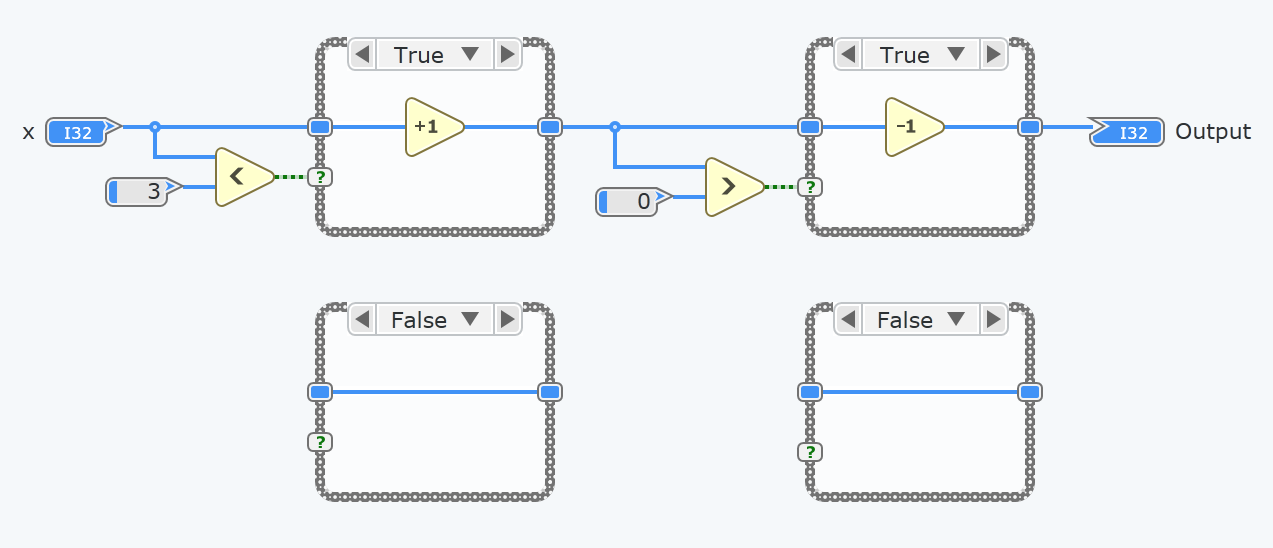
\includegraphics[width=150mm,keepaspectratio]{figures/testvi1.png}
\caption{Example VI "A"} 
\label{fig:testvi1}
\end{figure}

\begin{lstlisting}[frame=single,float=!ht,caption={The converted imperative version of VI "A"},captionpos=b,label={lst:testvi1_proc},language=]
A = [x]; 
B = 3; 
C = 0; 
D = (A < B); 
IF D Then
E = (A + 1); 
ELSE
E = A; 
End IF
F = (E > C); 
IF F Then
G = (E - 1); 
ELSE
G = E; 
End IF
[Output] : G; 
\end{lstlisting}


\begin{table}[]
\centering

\def\arraystretch{1.5}
\begin{tabular}{|l|l|l|}
\hline
           & \textbf{Path condition}                                         & \textbf{Calculated input values} \\ \hline
\textbf{1} & $x< 3\wedge x+1> 0$ & $x=0$                              \\ \hline
\textbf{2} & $x< 3\wedge \neg (x+1> 0)$ & $x=-1 $                            \\ \hline
\textbf{3} & $\neg(x< 3)\wedge x>0$ & $x=3$                     \\ \hline
\end{tabular}
\caption{Results of Demo A}
  \label{Tab:testvi1resu}
\end{table}
The outputs of symbolic execution in this example (Table \ref{Tab:testvi1resu}) are the same as the expected (see Figure \ref{fig:symbolic_test}), and the unreachable fourth execution path $(!([x] < 3) \& !([x] > 0))$ is omitted from the list.

To verify the correctness of the results, I ran the VI with these inputs, to see if they really produce different execution paths. As seen on Figure \ref{fig:verify1}, all the possible paths have been covered with this input set.
\begin{figure}
\centering
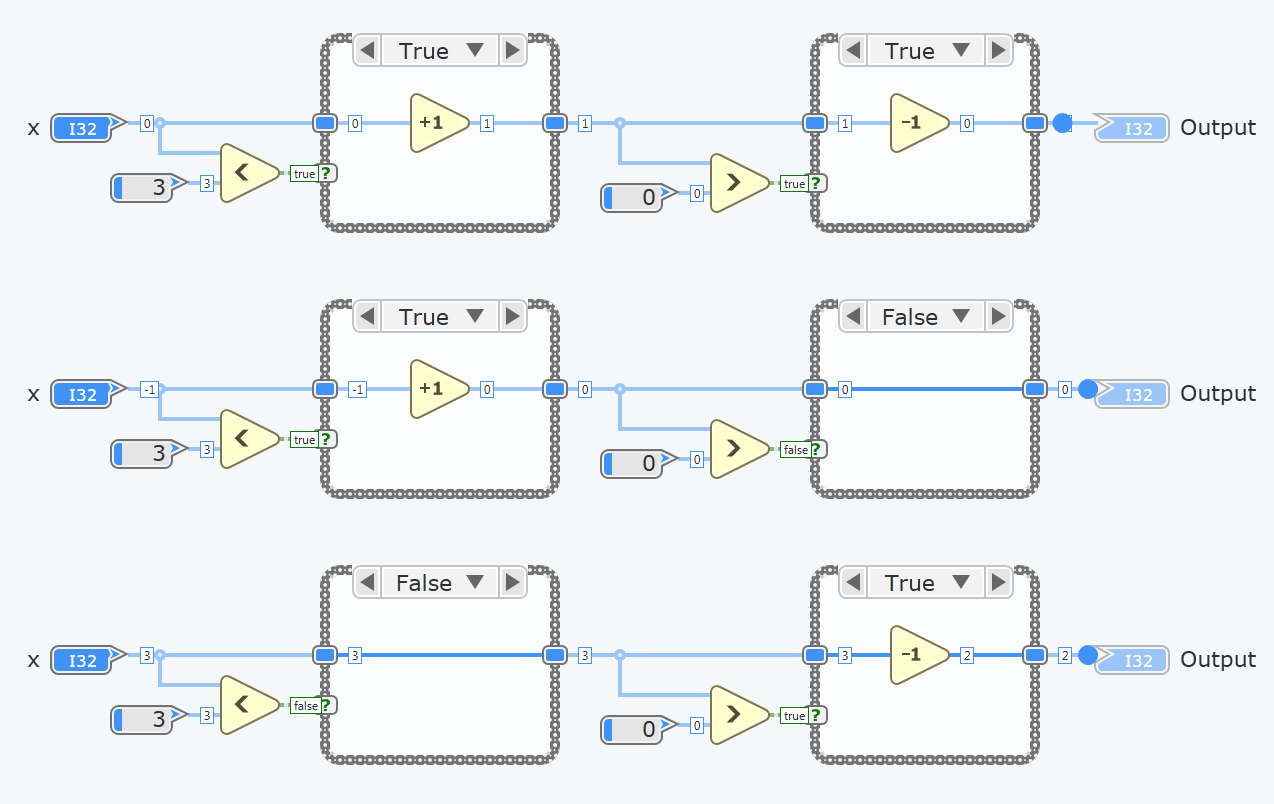
\includegraphics[width=140mm,keepaspectratio]{figures/verify1.png}
\caption{Run VI "A" with the result values as input} 
\label{fig:verify1}
\end{figure}

\paragraph{Demo "B"}
I wanted to test, if nesting case structures behaves correctly, therefore the second demo features nested structures (Figure \ref{fig:testvi2}). When \textit{outside var} is false, \textit{inside var} should not matter in the path condition. Additionally, this test verifies, that boolean input values are processed correctly.

\begin{figure}
\centering
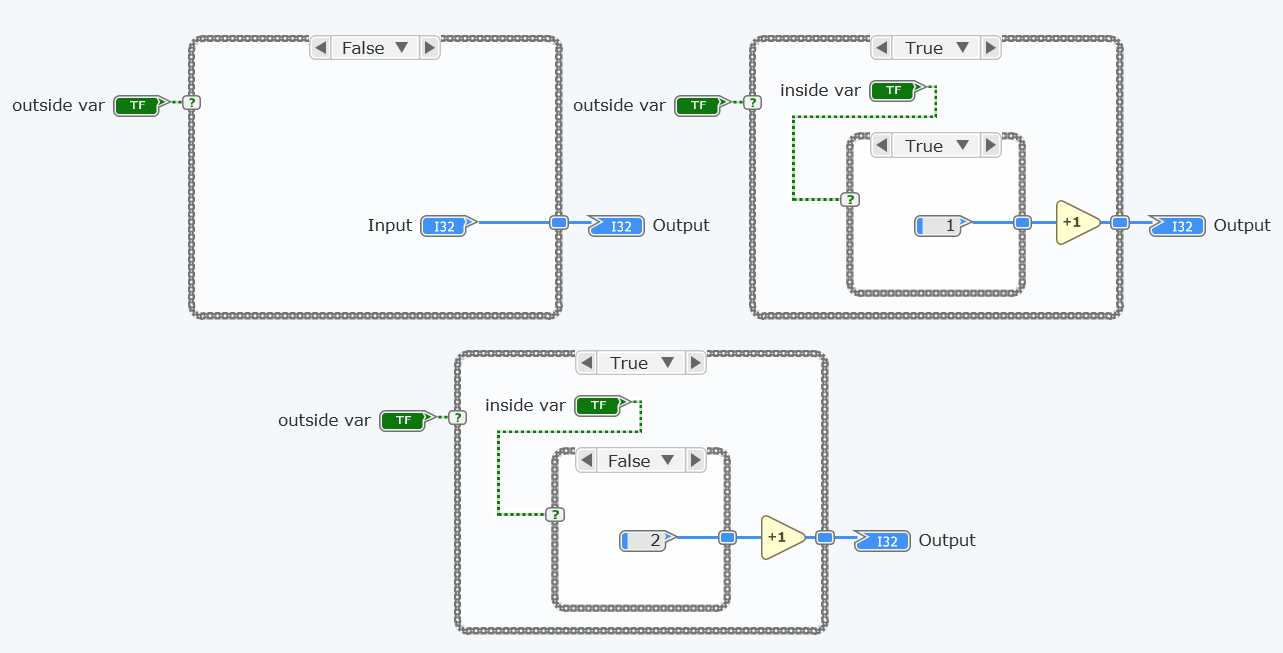
\includegraphics[width=150mm,keepaspectratio]{figures/testvi2.png}
\caption{Example VI "B"} 
\label{fig:testvi2}
\end{figure}


\begin{lstlisting}[frame=single,float=!ht,caption={The output of the symbolic execution for VI "B"},captionpos=b,label={lst:testvi2_sym},language=]
pc: ([outside var] & [inside var]), inside var=true, outside var=true
pc: ([outside var] & ![inside var]), inside var=false, outside var=true
pc: ![outside var], outside var=false
\end{lstlisting}
 % eredmenyek tablazatos formaban
\section{Results of testing}

% lista a tovabbi tesztesetekrol
I tested the tool with a number of other self-made VIs as input. Although there were bugs in some cases in the parser, when creating a certain pattern on the block diagram (resulting in an exception), the overall results indicate, that the tool is working correctly, and gives the correct outputs.

The tool runs on these simple VIs, almost instantaneously.


Since the prototype lacks support for more fundamental LabVIEW elements, unfortunately, I was unable to demonstrate it on a real-life application.

\begin{table}[ht]
\centering
\begin{tabularx}{\linewidth}{XX}
\toprule
\textbf{1. Return all possible paths (and path conditions) for VIs that have one or more case structures (with boolean conditions)}                         & The expected paths and inputs have been returned on the symbolic execution of Demo A, and the other VIs with a case structure                                           \\ \midrule
\textbf{2. Specify input variables for each path to be used to reach it}                                                                                    & Ran Demo A and other VIs with the specified values and highlighted execution: the execution paths were the same as the expected                                         \\ \midrule
\textbf{3. Return only one path for VIs without a case structure}                                                                                           & Test VI C with no case structure returned one line: "pc: True"                                                                                           \\ \midrule
\textbf{4. Support basic arithmetical, comparison and logical operations (+, -, *, ++, -{}-, \textless{}, \textgreater{}, ==, And, Or, Not) during execution} & These operations are all covered by the test VIs (see Table \ref{Tab:Trac}) \\ \midrule
\textbf{5. Support integer and boolean data types}                                                                                                          & The tested VIs work well with these data types, even if they are mixed in the symbolic variable set (Test D)                                                            \\ \midrule
\textbf{6. Stop execution of paths with an unsatisfiable condition}                                                                                         & Demonstrated by Demo A, the unsatisfiable path has been omitted                                                                                                         \\ \bottomrule
\end{tabularx}

\caption{Fulfilled requirements}
  \label{Tab:Requ}
\end{table}


The requirements specified in the Design chapter have been fulfilled, the creation of the prototype was successful.

\paragraph{Known bugs} If the tunnels of two nested subdiagrams are directly connected, the parser crashes, or gives wrong output. I was not able to fix that during the period of my BSc thesis.


% Please add the following required packages to your document preamble:
% \usepackage{multirow}
% Please add the following required packages to your document preamble:
% \usepackage{multirow}

\begin{table}[ht]

\def\arraystretch{1.8}
\centering
\begin{tabular}{lccccccc}
\hline
\multicolumn{2}{l}{\textbf{Requirement}} & \textbf{A} & \textbf{B} & \textbf{C} & \textbf{D} & \textbf{E} & \textbf{F} \\ \hline
\multicolumn{2}{l}{1.}             & \cmark          & \cmark          & \cmark          & \cmark          & \cmark          & \cmark          \\ \hline
\multicolumn{2}{l}{2.}             & \cmark          & \cmark          &            & \cmark          & \cmark          & \cmark          \\ \hline
\multicolumn{2}{l}{3.}             &            &            & \cmark          &            &            &            \\ \hline
          & +                     &            &            & \cmark          &            &            &            \\ \cline{2-8} 
          & -                     &            &            & \cmark          &            &            &            \\ \cline{2-8} 
          & *                     &            &            & \cmark          &            & \cmark          &            \\ \cline{2-8} 
          & ++                    & \cmark          & \cmark          &            & \cmark          &            &            \\ \cline{2-8} 
          & -{}-                    & \cmark          &            &            & \cmark          &            &            \\ \cline{2-8} 
4.         & \textless{}           & \cmark          &            &            &            &            &            \\ \cline{2-8} 
          & \textgreater{}        & \cmark          &            &            & \cmark          &            &            \\ \cline{2-8} 
          & ==                    &            &            &            &            & \cmark          &            \\ \cline{2-8} 
          & And                   &            &            &            &            &            & \cmark          \\ \cline{2-8} 
          & Or                    &            &            &            &            &            & \cmark          \\ \cline{2-8} 
          & Not                   &            &            &            &            & \cmark          & \cmark          \\ \hline
\multicolumn{2}{l}{5.}             & \cmark          & \cmark          & \cmark          & \cmark          & \cmark          & \cmark          \\ \hline
\multicolumn{2}{l}{6.}             & \cmark          &            &            &            &            &           \\ \hline

\end{tabular}

\caption{Traceability of requirements}
  \label{Tab:Trac}
\end{table}
%% screenshots